This is a lab that spanned two weeks and covered the design of security
architectures with securiCAD.

\section{Threat Model}
\label{s:threat-model}

\begin{figure}[H]
  \centering
  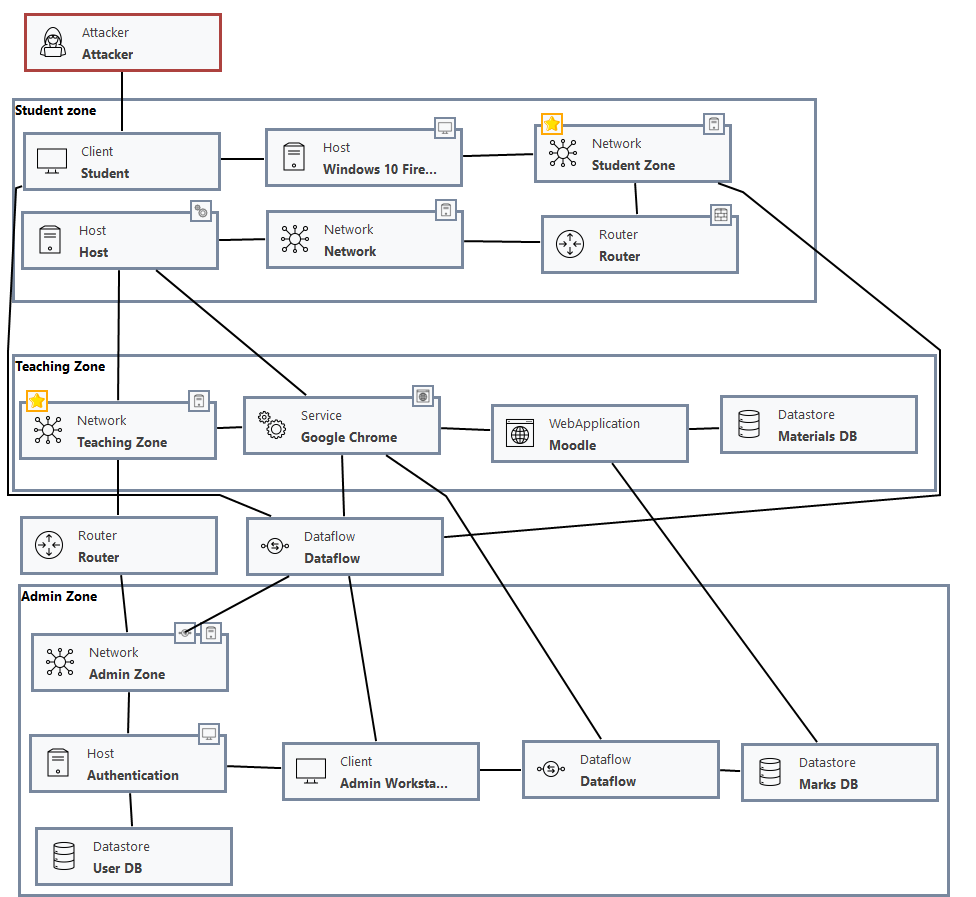
\includegraphics[width=1\textwidth]{figures/securiCAD}
  \caption{securiCAD Threat Model}
  \label{f:securiCAD-Model}
\end{figure}

The model created on securiCAD has been developed with the scenario that has
been given. The model is a set of three zones and routers figuratively placed
out of them. It follows a sort of pipeline where a user, in this case, a student,
can connect to his zone where through ACL implementation, can perform
operations such as access to the teaching zone. The student with access to
Moodle with a Browser and has access to the frontend that fetch data from a
database that requires special authorisations to be accessed and stores
important data such as lectures, timetables, marks, tests and more. The teaching
zone is attached to the Admin Zone through a router that performs authentication.
When authenticating, if the role is admin, the account will have the power to
send mutations queries to the database and modify tables.
The targets that I've chosen for the attack are the student zone with a
compromise attack step and the teaching zone with an attack step of Denial of
Service.

\begin{figure}[H]
  \centering
  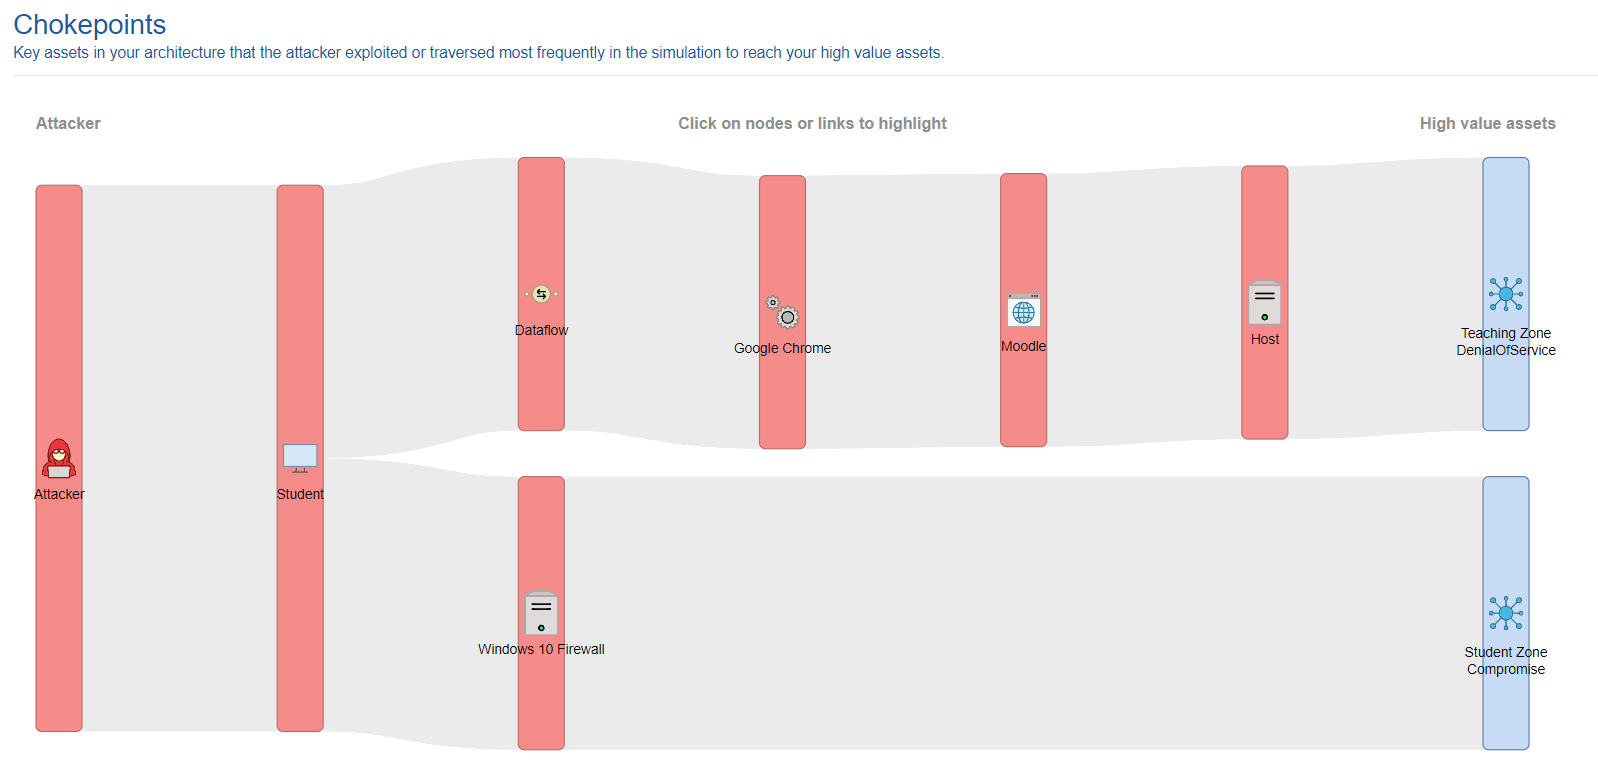
\includegraphics[width=1\textwidth]{figures/chokepoints}
  \caption{Chokepoints}
  \label{f:chokepoints}
\end{figure}
The image above shows the critical assets in the architecture and the workflow
pipeline that the attacker is using to compromise it. The high-value assets of
the simulation are the Student Zone and Teaching zone, with an attack
probability of 100\% and high risk.

\begin{figure}[H]
  \centering
  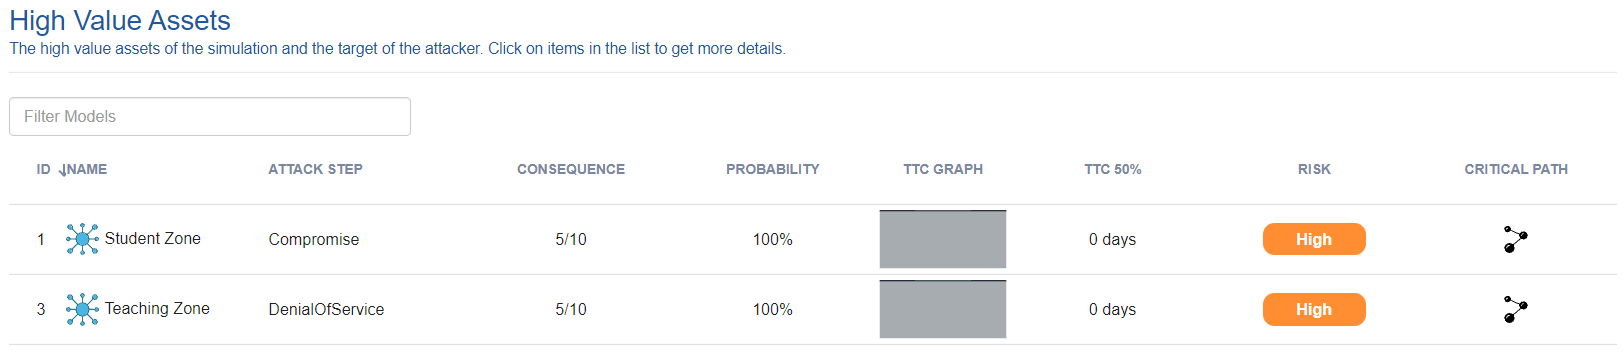
\includegraphics[width=1\textwidth]{figures/key-assets}
  \caption{Key Assets}
  \label{f:key-assets}
\end{figure}

The overall total risk expose shown in the securiCAD report is 100\%, meaning
that the architecture is very susceptible to attacks.

\begin{figure}[H]
  \centering
  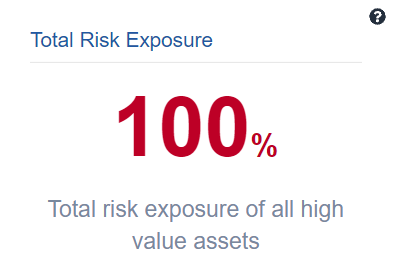
\includegraphics[width=0.4\textwidth]{figures/risk-exposure}
  \caption{Risk Exposure}
  \label{f:risk-exposure}
\end{figure}

After analysing the model, many changes to the architecture are required to
make it much more secure. Encryption could be one of the first solutions within
the network to make life a bit harder for a potential attacker.

To strengthen the most sensitive parts of the network, Network Segmentation
could also come to play. It would create dead ends for the attacker and a sort
of maze that would confuse and make his life harder, coupled with robust access
control and monitoring of user systems with firewalls.
